\section{Evaluation}
\label{sec:evaluation}

%This section describes our experimental design and the evaluation results.

\subsection{Comparison Method}

We compare our method with \emph{Brute Force}---measures all possible configurations and \emph{CherryPick}---the state-of-the-art method
~\cite{Alipourfard2017}.
Besides, we use  \emph{Random-4} and \emph{Random-8}, which randomly measures 4 and 8 configurations (for each workload) respectively as straw man methods.
The comparison metrics are  \emph{measurement cost} and \emph{search performance}.

The \emph{brute force} approach needs to test each configuration, and therefore, it generates constant measurement cost ($|S_w| \times |W|$).
The measurement cost of CherryPick varies for different workloads since it uses a heuristic stopping criterion. The lower bound is $3\times |W|$ because CherryPick uses at least three measurements as its initial points.
\micky performs collective optimization, and hence the measurement cost is shared by a batch of workloads and therefore, expected to be much lower than the other methods.

To compare their search performance, we use normalized performance in terms of execution time (the elapsed time required to complete a workload) and operational cost (the charge for completing a workload).
The \emph{brute force} approach always finds the optimal configuration while
the CherryPick is very likely to find near-optimal choices.
We examine whether \micky can find near-optimal configurations that are comparable to the \emph{CherryPick} approach.
A method delivers better search performance when the performance of found solutions is closer to the optimal.
For example, $1.05$ is better than $1.15$ because the former is only 5\% slower than the optimal.

We demonstrate the effectiveness of \micky using 107 workloads on Apache Hadoop and Spark.
These workloads are representative of many real-world applications.
Table~\ref{table:dataset} lists a subset of the workloads.
Please refer to our previous work for more details~\cite{Hsu2018Arrow, Hsu2018Scout, scoutdataset}.


\iffalse
\begin{figure}[t]
 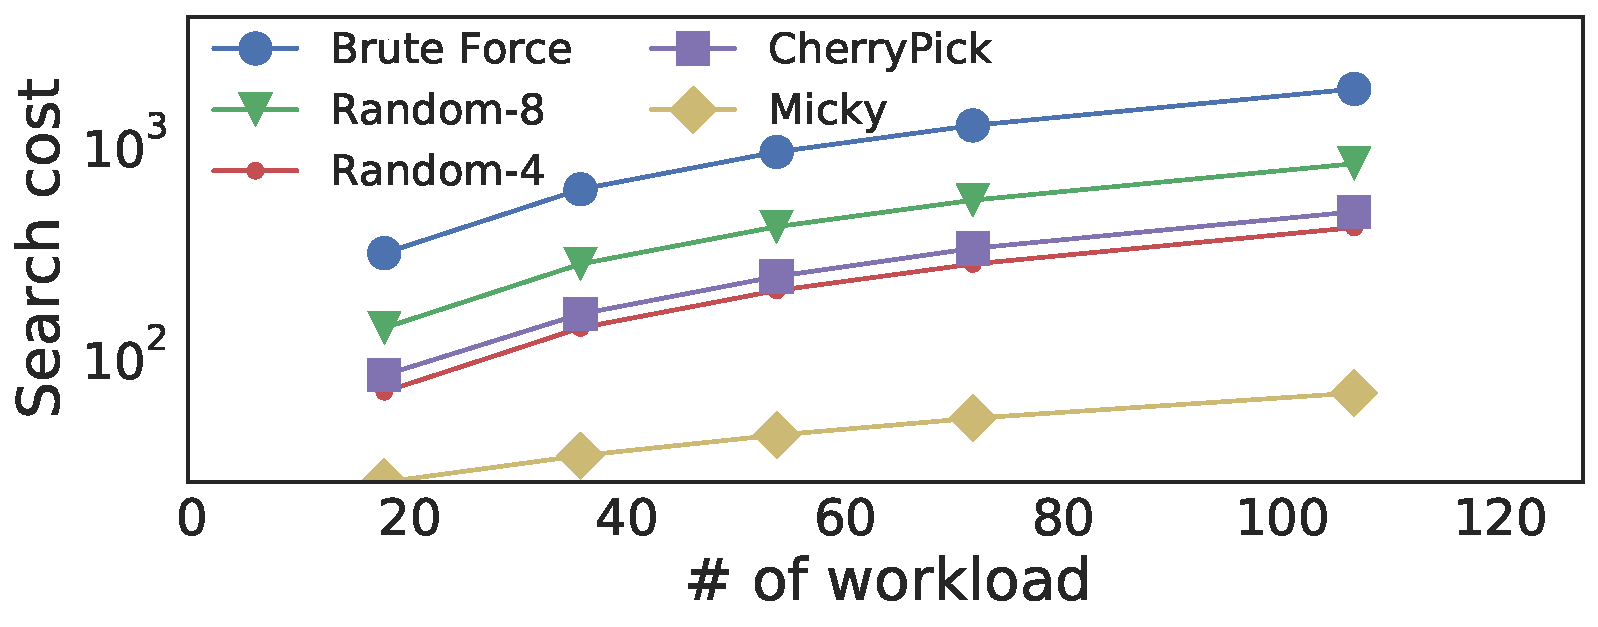
\includegraphics[width=.4\textwidth]{Figures/s0_single_time_steps_sum.pdf}
 \centering
 \caption{\textbf{Growth of measurement cost.} \micky is more economic when the number of workloads increases.  When the budget for optimization is limited, collective optimization becomes more promising.}
 \label{fig:scalability}
\end{figure}
\fi



\subsection{Experiment Setup}
\label{sec:setup}

%We list the parameters used in \emph{CherryPick} and \micky. 

\subsubsection*{CherryPick---Bayesian Optimization}

We encode the cloud configurations (\ie{CPU types, core counts, memory size per code and the bandwidth to Elastic Block Storage}) to represent the search space.
For the parameters, we choose the same kernel function (\emph{Mat\'ern 5/2}) and
the same stopping criteria (\textbf{EI}=10\%), as used in \emph{CherryPick}.
Regarding the choice of initial points, we randomly select three cloud configurations.
The above process is repeated 100 times for reducing artifact and better showing the capability of \emph{CherryPick}.


\subsubsection*{\micky---Multi-Armed Bandit}
There are three common algorithms for the multi-armed bandit problems as described in Section~\ref{sec:mab}.
We choose UCB because it is more stable as compared to other bandit algorithms
(will be discussed later in Section~\ref{sec:tuning_mab}).
\micky runs in two phases: (1) pure exploration, and (2) exploration along with exploitation.
In the pure exploration phase, \micky measures the performance of VMs with random workloads for improving stability and reduces sampling bias.
The $\alpha$  parameter represents the number of exhaustive iterations over each VM type.
In the second phase, \micky runs the algorithm to handle the exploration and the exploitation.
The behavior of this phase is controlled by the parameter $\beta$, which controls the number of measurements for finding the exemplar configurations.
The measurement cost of \micky is $(\alpha \times \mathit{|S|} + \beta \times \mathit{|W|}$).
We have observed that the measurement cost is directly proportional to the effectiveness of \micky.
In our experiments, we choose $\alpha=1$ and $\beta=0.5$.



\subsection{Can \emph{Micky} identify the exemplar cloud configurations?}

The primary goal of \micky is to find the most suitable cloud configuration across all workloads.
In this evaluation, we show the search performance in finding the cost-effective VM types.
In Figure~\ref{fig:s2_cost_performance}, we use box plot for comparison.
The red line in the box represents the median value while the two sides of the box are the first and third quartile.
The whiskers represent the 10 and 90 percentile respectively.

From this figure, we observe that the performance of \micky is comparable to CherryPick in the majority of workloads (using the median).
\micky is only 5\% worse than CherryPick on Spark 2.1 and Spark 1.5.
Surprisingly, \micky is slightly better than CherryPick on Hadoop 2.7.
The variance of \micky is higher because \micky
optimizes most workloads but fails to optimize for some.
We will discuss how to remedy this situation in Section~\ref{sec:system}.

To explain why \micky works, we further analyze the exemplar VM types recommended by \micky as listed in \mytable{\ref{table:top3}}.
The table shows the percentage of workloads that are within the performance thresholds.
CherryPick finds good VM types ($< 1.2$) in 86\% of workloads while
\micky achieves the same search performance performance in 71\% of workloads using only 11.6\% of measurements by CherryPick.

% Please add the following required packages to your document preamble:
% \usepackage{booktabs}
\begin{table}[!htbp]
\centering
\caption{\textbf{The most cost-effective VM types  for 107 workloads recommended by \micky} The number above each column label represents normalized performance (to the optimal). CherryPick finds good ($< 1.2$) VM types in 86\% of workloads.}
\label{table:top3}
\begin{tabular}{@{}lp{2cm}p{2cm}p{2cm}p{2cm}p{2cm}@{}}
\toprule
& $= 1.0$ \newline \textbf{Optimal}   & $< 1.1$ \newline \textbf{Excellent} & $< 1.2$ \newline \textbf{Good} & $\le 1.4$ \newline \textbf{Tradeoff} & $> 1.4$ \newline \textbf{Unsettled}     \\ \midrule
c4.large  & 48\%      & 61\% & 66\%      & 70\%        & 30\% \\
m4.large  & 27\%      & 46\% & 71\%      & 84\%        & 16\% \\
m4.xlarge & 9\%       & 15\% & 32\%      & 63\%        & 37\% \\ \bottomrule
\end{tabular}
\end{table}


\subsection{When not to use \micky?}
\label{sec:kneepoint}

\micky reduces measurement cost while delivering satisfactory performance.
However, there exists a trade-off between the cost reduction achieved by \micky and its effectiveness.

First, \myfigure{\ref{fig:cost_saving}} shows that \emph{CherryPick} is four times expensive than \micky. As the number of workloads increases, \micky is more economical because
the cost of pure exploration phase of \micky remains constant. This is because $\alpha$ depends only on the number of cloud configurations.
We observe that \micky only uses a fraction of the measurement cost when compared to the other methods.
For example, when optimizing for 40 workloads, \micky only uses 30 measurements to find the suitable cloud configuration whereas CherryPick uses 156 measurements.
Another observation is that \micky is more scalable because the slope of the line decreases as the number of workloads increases.

\begin{figure}[!htbp]
 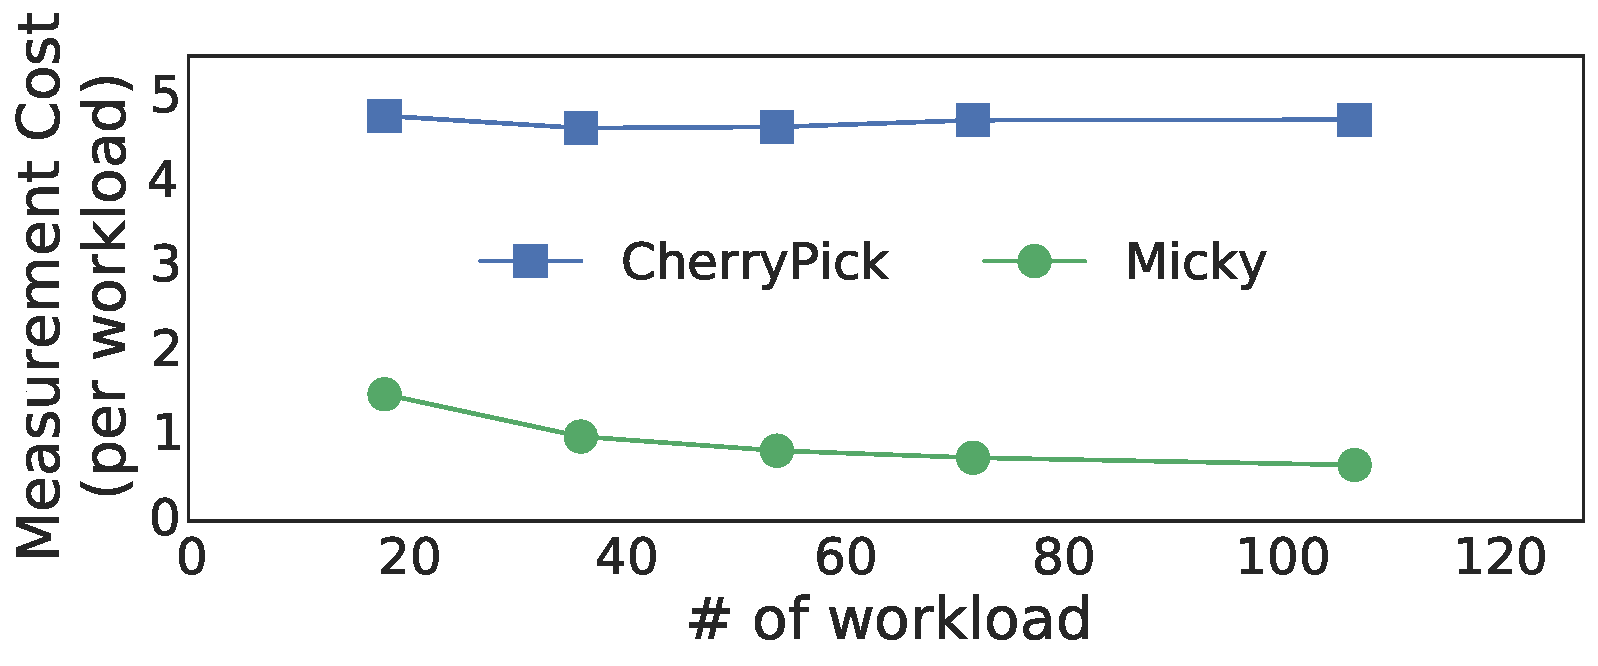
\includegraphics[width=.8\textwidth]{Figures/s0_single_time_steps_comparison.pdf}
 \centering
 \caption{\textbf{Low measurement cost in collective optimization.} \emph{CherryPick} optimizes each workload separately while \micky finds the exemplar cloud configuration suitable for a group of workloads.}
 \label{fig:cost_saving}
\end{figure}

Second, a user demands near-optimal solutions (\eg{$<1.1$})
mostly for highly recurring workloads because its measurement cost can be amortized.
In \mytable{\ref{table:break_even_cost}}, we show the \textit{knee-point} that a user should use a single-optimizer rather thatn a collective-optimizer.
We calculate the knee point using
$K \times f(\Delta_{P}, C_{P}) \ge g(\Delta_{M}, C_{M})$,
where $K$ is the recurrence of a workload as the knee point,
the function $f$ represents the opportunity loss due to inferior search performance, and
the function $g$ represents the reduction of measurement cost when using collective optimization.
In addition, 
$\Delta_{P}$ is the delta of normalized search performance (between a single- and collective-optimizer),
$\Delta_{M}$ is the delta of measurement cost.
$C_{P}$ and $C_{M}$ are cost (\eg{dollars}) defined by users.
For simplification, we use $C_{P} = 10 \times C_{M}$ in this calculation..
For non-critical workloads (\eg{recurring batch-process jobs}),
$C_{P}$ is lower, and hence, \micky is more beneficial.
As shown in \mytable{\ref{table:break_even_cost}},
\emph{CherryPick} is preferred only when
the same workloads run more than 20 to 30 times.
Otherwise, \micky is a more desirable solution.

% Please add the following required packages to your document preamble:
% \usepackage{booktabs}
\begin{table}[!htbp]
\centering
\caption{\textbf{The knee point when \micky should not be used.} 
The knee point (the number of recurrence of workloads) represents a trade-off between search performance and measurement cost.
}
\label{table:break_even_cost}
\begin{tabular}{@{}llllll@{}}
\toprule
            & 18   & 36    & 54   & 72   & 107  \\ \midrule
Brute Force & 84.8 & 120.6 & 55.0 & 52.1 & 57.3 \\
Random-8    & 37.9 & 51.5  & 33.7 & 36.0 & 44.7 \\
Random-4    & 18.4 & 24.2  & 27.0 & 28.5 & 27.9 \\
CherryPick  & 23.3 & 30.8  & 20.8 & 24.0 & 27.0 \\ \bottomrule
\end{tabular}
\end{table}


\begin{figure}[!htbp]
 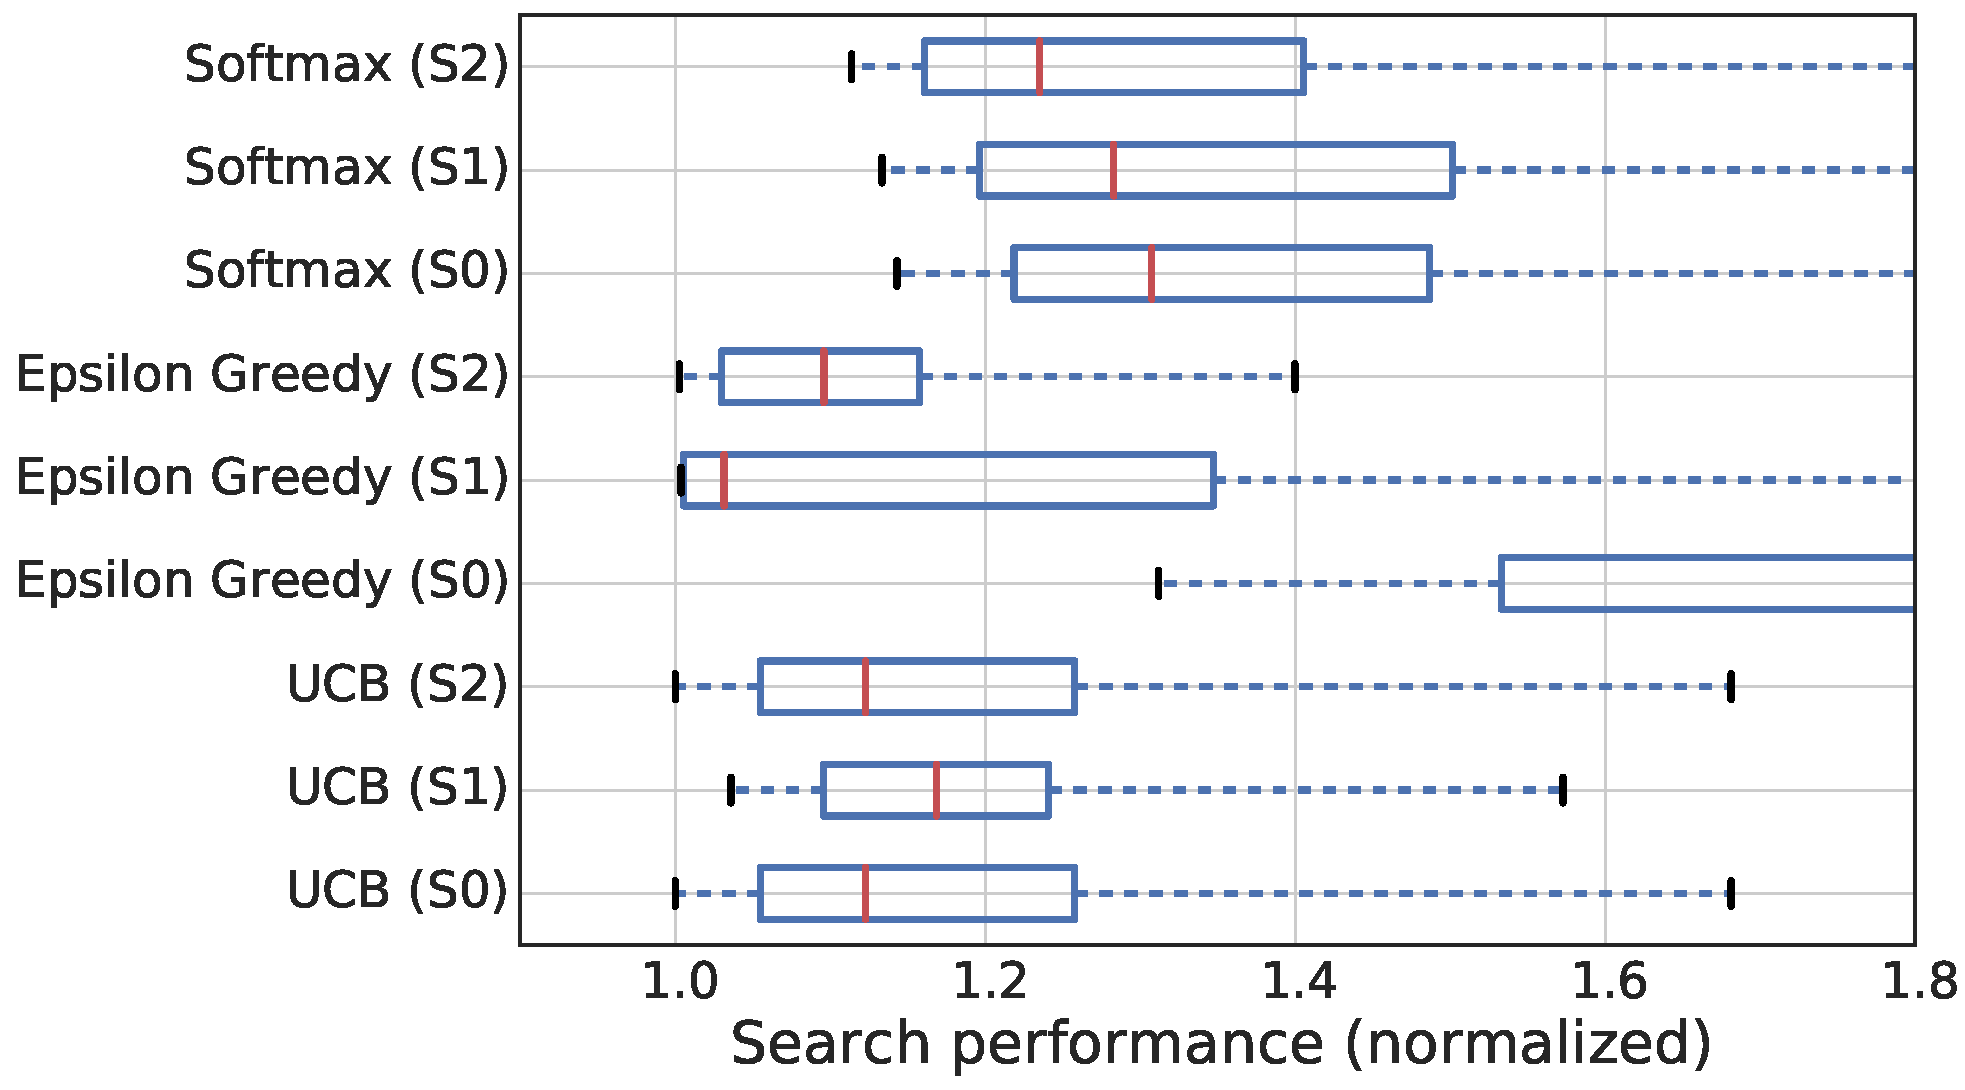
\includegraphics[width=.8\textwidth]{Figures/s0_single_algorithm_selection.pdf}
 \centering
 \caption{\textbf{Selection of multi-armed bandit algorithms.} The parameter (in the parenthesis) controls the measurement budget ($S0 < S1 < S2$).}
 \label{fig:algorithm_selection}
\end{figure}

\subsection{Why UCB is the preferred choice?}
\label{sec:tuning_mab}

To select the suitable method for \micky, we compare three multi-armed bandit algorithms
(as mentioned in Section~\ref{sec:methods}).
First, the behavior of Epsilon Greedy is controlled by the parameter $\epsilon$. A larger value encourages exploration while a lower value encourages exploitation.
We choose 0.1 for the epsilon parameter.
Second, the Softmax algorithm uses a temperature parameter for structured exploration.
The Softmax algorithm with an infinity temperature uses pure exploration while a zero value sticks to the arm (cloud configuration) with the highest estimated probability---pure exploitation.
We use 0.1 for the temperature parameter.
Last, the Upper Confidence Bound algorithm (UCB) tracks the confidence of rewards of arms.
There are no parameters.

\myfigure{\ref{fig:algorithm_selection}} presents the comparison between the three methods.
The parameter in the parenthesis represents the measurement budget, determined by $\alpha$ and $\beta$ (as described in Section~\ref{sec:setup}).
We choose 0, 1, 2 as the $\alpha$ parameter for $S0, S1, S2$ and use 0.5 for $\beta$ in all.
This figure shows UCB is more stable.
Besides, the performance of UCB does not heavily rely on parameter tuning.
Therefore, we prefer UCB to Epsilon Greedy, and \micky is built using UCB.





\begin{figure}[!htbp]
 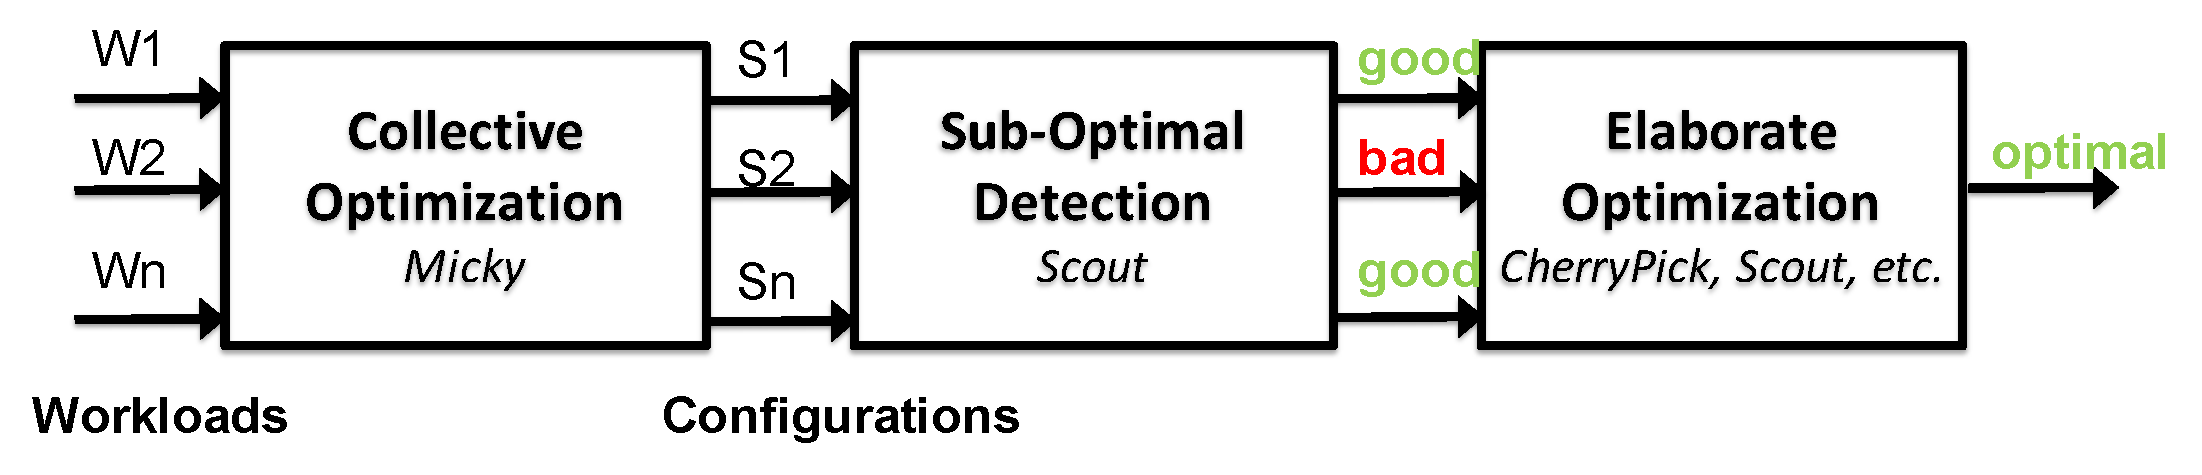
\includegraphics[width=.8\textwidth]{Figures/system_integration.pdf}
 \centering
 \caption{\textbf{A system integration to alleviate sub-optimal choices in some workloads.} \scout answers ``is there a better configuration than the current choice?''~\cite{Hsu2018Scout}. An integration of \micky and \scout delivers a more efficient and reliable recommendation system of cloud configurations.}
 \label{fig:system_design}
\end{figure}


\begin{figure}[!htbp]
 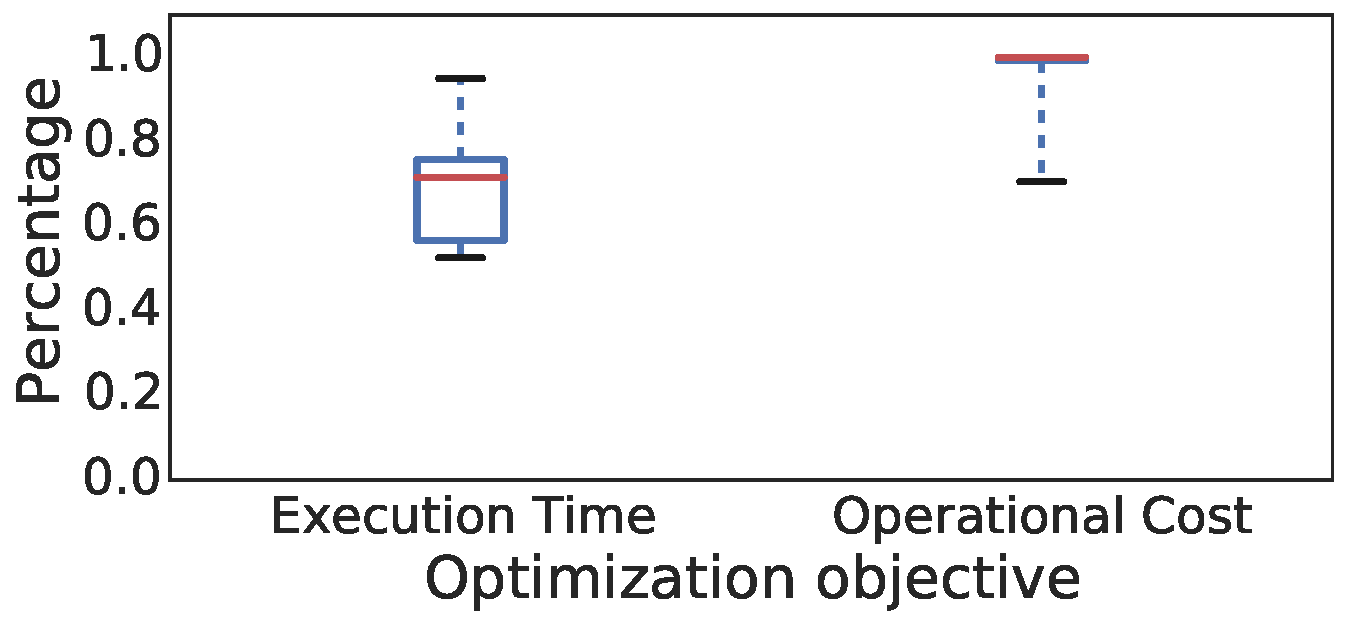
\includegraphics[width=.8\textwidth]{Figures/s4_misprediction_correction.pdf}
 \centering
 \caption{\textbf{Detection of mis-predictions using \scout.} The percentage represents the truth positive ratio, the probability the unsettled configurations can be identified.  The two optimization objectives are to find the fast configuration and the most cost-effective VM type respectively.}
 \label{fig:detection_misprediction}
\end{figure}